\documentclass[a4paper,10pt]{article}
\usepackage[utf8]{inputenc}
\usepackage{amsmath}
\usepackage{amssymb}
\usepackage{graphicx}
\graphicspath{ {images/} }
% \usepackage {tikz}
% \usetikzlibrary {positioning}
% \definecolor {processblue}{cmyk}{0.96,0,0,0}
% 
% \usetikzlibrary{chains,shapes.multipart}
% \usetikzlibrary{shapes,calc}
% \usetikzlibrary{automata,positioning}
% 
% \tikzset{
% buffer/.style={
%     draw,
%     shape border rotate=270,
%     regular polygon,
%     regular polygon sides=3,
% %       fill=red,
%     node distance=2cm,
%     minimum height=4em
%  }
%  }



% Title Page
\title{Online Learning of Hitting Time of Markov Chains}
\author{Chandramouli K}
\date{May 2, 2016}

\begin{document}
\maketitle
\section*{Motivation}
In general, wireless communication networks have a source and target connected through 
many channels, unreliable due to noisy surroundings. In such a case a scheduler wishes to 
transmit data quickly through the ``most reliable'' channel among the channels available.  
This task of choosing ``most reliable `` channel becomes difficult when probabilistic model 
information of these channels is unknown. In this project we address this problem of 
scheduling by learning the model information of the channels through sampling.
\section*{Model}
We model the wireless communication network as a multi-armed Markov bandit problem. Time is 
slotted $t= 1,2, \cdots T.$ Each channel is an arm assumed to be a Markov chain with unknown 
transition probability matrix and state space $S=\{0,1\}$ where 0 corresponds to channel being
inactive and 1 corresponds to channel being active. Suppose there are $m$ channels in the 
network then we have $m$  Markov chains $X^{i}_{t}, i=1,2, \cdots m, t \in \mathbb{N},$ taking 
values in $\{0,1\}.$ At time instant $t$ the scheduler chooses the arm (channel) 
$I_t \in [m]$ and observes the states $X^{i}_{t}, i=1,2, \cdots m.$ If $X^{I_t}_{t}=1$ then
scheduler has chosen an active channel and the transmition is successful. If $X^{I_t}_{t}=0$ 
then based on the observations $X^{i}_{t}, i=1,2, \cdots m$ the scheduler chooses $I_{t+1}.$
Let hitting time of state 1, $\tau$, be defined as $\tau := \min\{t:X^{I_t}_{t}=1\}.$ Our 
objective is to find a scheduling scheme that minimizes the expected hitting time of state 1.

%\section*{Algorithms}

\section*{Experiments}
To analyze this problem we employed the well known Thompson sampling algorithm for 
multi-armed bandit problems. We compared it with an algorithm that chooses 
$I_t \in [m]$ uniformly at random, with an algorithm that
chooses $I_t$ based on transition probability estimates formed from sample trajectories till
time $t-1$ and with an algorithm that chooses $I_t$ when transition probabilities are known.
The details of the experiments are summarised in the plot given below.
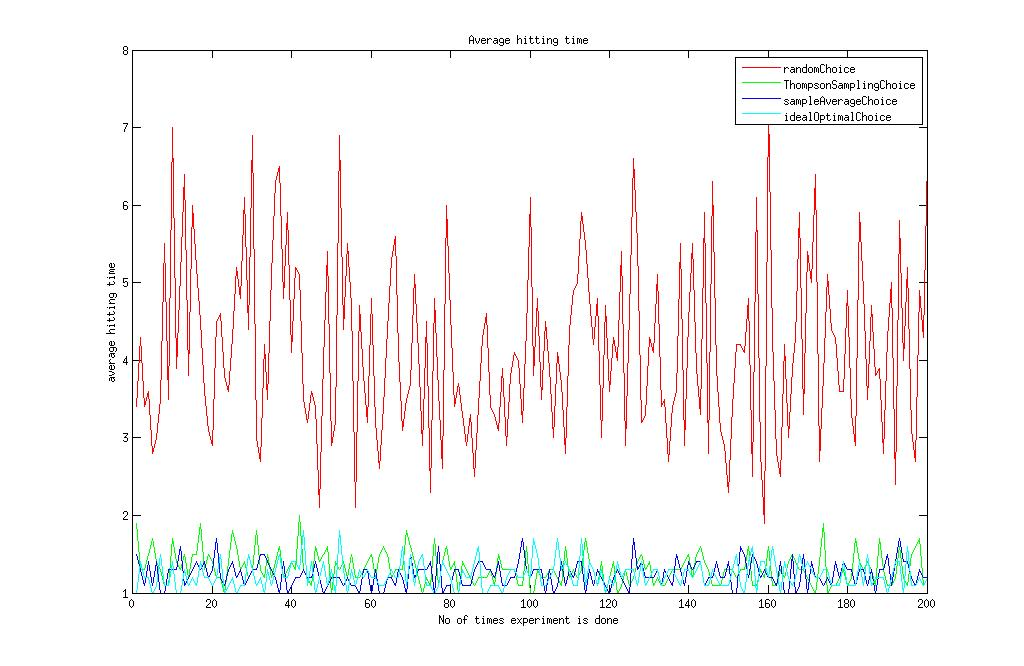
\includegraphics[width=100mm,scale=1]{AllObservationsKnownResult}
\section*{Conclusion}
To our surprise we find that simple sample trajectory based algorithm performs as well as
Thompson sampling for multi-armed bandit problems.
\nocite{*}
\bibliographystyle{ieeetr}
\bibliography{references}
\end{document}          
